
\documentclass[a4paper, 12pt]{article} % Define the type of document and formatting

\usepackage[utf8]{inputenc} % Allows for special characters
\usepackage{graphicx} % For including images
\usepackage{amsmath} % For mathematical symbols
\usepackage{hyperref} % For hyperlinks
\usepackage{geometry} % For page layout
\geometry{margin=1in} % Adjust margins



\begin{document}


\section{\textbf{\LARGE Requirement Analysis}}
\subsection{\textbf{\Large Introduction}}
In this context of requirement analysis, the ElderCare Connect Progressive web application is designed to meet the needs of specific users such as elderly people and caregivers. The primary focus of the requirement analysis is to define the functional and non-functional requirements of the system. User requirements of the application include Health monitoring, Emergency Response and social engagement and  the non-functional requirements include Performance, usability, reliability, security, scalability, maintainability and availability.

\subsection{\Large User Requirements} 

\textbf{\large Elderly Users} 
\begin{itemize}
    \item \textbf{Health Monitoring:} Integration with wearable devices to track vital signs like heart rate, blood pressure, and physical activity. 
    \item \textbf{Emergency Alerts:} Automatic fall detection and an SOS button for emergencies, sending alerts to family, caregivers, or emergency services.
    \item \textbf{Medication Reminders:} Notifications to take prescribed medications, reducing the risk of missed doses. 
    \item \textbf{Daily Check-ins:} Gentle reminders for users to confirm their well-being or complete a wellness survey.
    \item \textbf{Social Engagement:} Messaging, and virtual communities to reduce isolation and encourage interaction.
\end{itemize}
\textbf{\large Caregivers/family} 
\begin{itemize}
    \item \textbf{Real-time Alerts:} Immediate notifications for falls, emergencies, or missed check-ins.
    \item \textbf{Health Reports:} Weekly or monthly health reports with trends in the user's vital stats, activity levels, and overall well-being.
    \item \textbf{Location Tracking:} Real-time GPS tracking during emergencies or to ensure the user's safety.
    \item \textbf{Communication Tools:} Instant messaging to check on the elderly user.
\end{itemize}

\subsection{Users}
\begin{enumerate}
    \item Caregivers/family
    \item Elderly Users
\end{enumerate}

\subsection{Functional Requirements}
\textbf{Health Monitoring }
\begin{itemize}
    \item The app will be able to synchronize and connect with wearable devices as well as health monitoring platform, Google Fit (Android) which are designed to monitor the heart rate of users, their activity, etc. sleep patterns, their activity levels etc. This data shall be monitored over the internet and in case of any abnormalities such as a distinct drop in heart rate or a fainting episode, alerts will go off. [1]
\end{itemize}
\textbf{Emergency Response}
\begin{itemize}
    \item In the event of a medical emergency or situation where a patient falls, the app shall send push notifications to the emergency contacts or the caregivers who are predesignated. It is also possible for the users to use the emergency call function (with the help of a REST API) in case they feel the need for help or are unwell.
\end{itemize}
\textbf{Social Engagement }
\begin{itemize}
    \item Recognizing the significance of social engagement, which is crucial in enhancing the well-being of the elderly, the only such application will integrate a number of features such as instant messaging where old or elderly users can meet family members, caregivers, which will help in alleviating loneliness and associated feelings. If the elderly member is in danger this features a location sharing technique to send their location to their cared ones. This also allows the family members and caregivers to remind their lovely one’s medications, hydrations and medical consultations simply contact with them.
\end{itemize}
\subsection{Non-functional Requirements}
\textbf{Performance: }
\begin{itemize}
    \item The app should provide real-time monitoring and instant emergency alerts within 2 seconds of a triggering event 95\% of the time, especially during critical moments like falls or health issues.
    \item It should handle multiple users and real-time data input from up to 100,000 wearable devices effectively, maintaining response time of under 1 second per device.
\end{itemize}
\textbf{Usability }
\begin{itemize}
    \item The user interface should be simple and intuitive, designed with large fonts (minimum size 18pt) and easy navigation, particularly catering to elderly users with minimal technical experience (new users will be able to locate easily the primary functions such as emergency alerts, health stats, and alerts within 2 seconds).
    \item The app must be highly reliable to ensure constant monitoring and timely emergency alerts, at least 99.9\% uptime.
    \item Emergency alert mechanisms should function with at least 98\% accuracy, even in low connectivity scenarios (1 Mbps).
\end{itemize}
\textbf{Security }
\begin{itemize}
    \item Data privacy and security are critical, especially since the app deals with sensitive health information. The app must comply with healthcare privacy regulations like HIPAA (or regional equivalents) to protect user data as well as Personal Data Protection Act (PDPA).
    \item Secure login and role-based access for family members and caregivers to ensure only authorized individuals can view the elderly user's health data.
\end{itemize}
\textbf{Scalability }
\begin{itemize}
    \item The back-end should support future scalability as 100\% increase in users and data volume within one year without affecting performance metrics, handle up to 5 million records allowing additional data points (such as vital signs) as needed.
\end{itemize}
\textbf{Maintainability }
\begin{itemize}
    \item The system should be easy to update with new features or improvements, such as new integrations with different wearable devices or additional health monitoring features with maximum downtime of 5 minutes per update.
\end{itemize}
\textbf{Availability }
\begin{itemize}
    \item The system must ensure high availability, especially during emergencies, and maintain uptime for 24/7 real-time monitoring.
    \item Regular maintenance or updates should not interfere with the core emergency functionalities.
\end{itemize}
\textbf{Privacy and Security }
\begin{itemize}
    \item As the application deals with sensitive personal health information, the app will definitely put in place stringent measures such as the use of JWT (JSON Web Tokens) for user validation and SSL which encrypts data during transfer. Such measures go a long way in securing personal health information.
\end{itemize}
\subsection{UseCase Diagram}
\begin{figure}
    \centering
    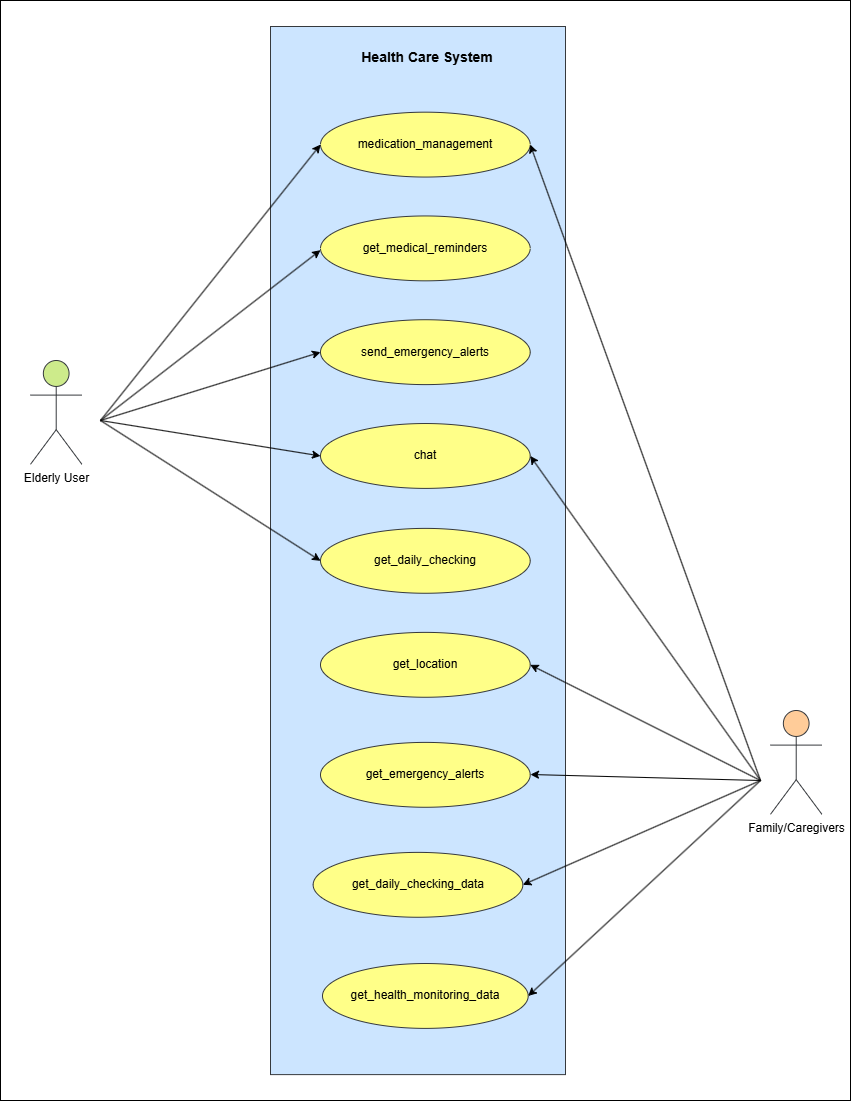
\includegraphics[width=0.5\linewidth]{usecase3.drawio (1).png}
    \caption{Enter Caption}
    \label{fig:enter-label}
\end{figure}
\end{document}

